\documentclass[10pt]{beamer}
\usetheme{AGH}

\usepackage{lmodern}
\usepackage[utf8]{inputenc}
\usepackage{listings} 
\usepackage{siunitx}
\usepackage{filecontents,hyperref}
\usepackage{graphicx}
\usepackage{subcaption}
\usepackage{svg}

\usepackage{appendixnumberbeamer}
\usepackage{booktabs}
\usepackage{xspace}
\newcommand{\themename}{\textbf{\textsc{metropolis}}\xspace}


\title{}
\subtitle{\normalsize{Tasks undertaken as part of the engineering thesis}}
\date{17\textsuperscript{th} February 2020}
\author{\normalsize{Arkadiusz Kasprzak \newline \and Jarosław Cierpich \newline \and Grzegorz Podsiadło \newline \newline \and Supervisor: Bartosz Mindur}}



\lstdefinestyle{custom}{
  breaklines=true,
  frame=single,  
  language=[ISO]C++,
  basicstyle=\ttfamily\tiny,
  keywordstyle=\color{blue},
  commentstyle=\color{orange},
  numbers=left,                  
  numbersep=5pt,   
  literate={ą}{{\k{a}}}1
           {Ą}{{\k{A}}}1
           {ę}{{\k{e}}}1
           {Ę}{{\k{E}}}1
           {ó}{{\'o}}1
           {Ó}{{\'O}}1
           {ś}{{\'s}}1
           {Ś}{{\'S}}1
           {ł}{{\l{}}}1
           {Ł}{{\L{}}}1
           {ż}{{\.z}}1
           {Ż}{{\.Z}}1
           {ź}{{\'z}}1
           {Ź}{{\'Z}}1
           {ć}{{\'c}}1
           {Ć}{{\'C}}1
           {ń}{{\'n}}1
		   {Ń}{{\'N}}1
}


\begin{document}

\maketitle

\begin{frame}
\frametitle{Agenda}
\tableofcontents
\end{frame}

\begin{frame}{New project architecture}
Characteristics of the new project architecture:
\begin{itemize}
	\item Every module does only need minimal required dependencies to compile
	\item New architecture does bring valuable information about dependencies in the project and inter-module interactions
	\item Modules has been hierarchized. There are hierarchy levels and dependencies point only towards the lower level of hierarchy.
\end{itemize}
\end{frame}

\begin{frame}{New project architecture}
\begin{figure}
\centering
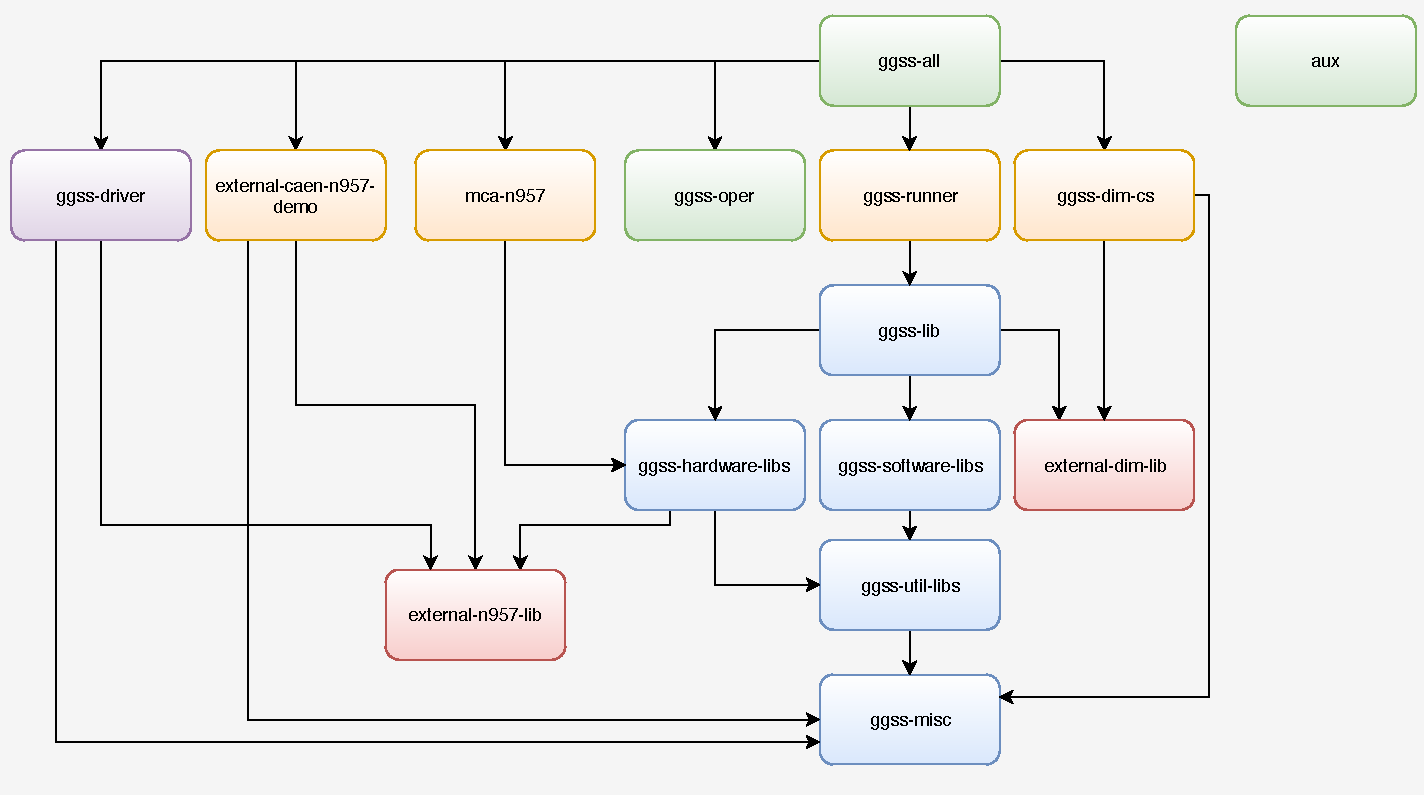
\includegraphics[width=\linewidth]{resources/topLevelArchitecture}
\caption{Architecture of the GGSS project}
\end{figure}
\end{frame}

\begin{frame}{Migration to GIT}
\begin{itemize}
	\item Project has been migrated to GIT version control system. Every module has been divided into separate repository. Submodule feature has been used to achieve hierarchical structure and support fast setup of development environment.
	\item \textbf{atlas-trt-dcs-ggss} group has been created within which 20 repositories has been created.
	\item Issues, Milestones and Kanban Board are being used to organize and track work throughout development.
\end{itemize}
\end{frame}

\begin{frame}{Resources}
\begin{minipage}{0.65\linewidth}
	Following resources has been used to establish building environment:
	\begin{itemize}
		\item GitLab CERN resources - to run CI/CD on every single repository except ggss-driver which requires control over installed kernel version
		\item OpenStack CERN resources - to run CI/CD for ggss-driver
	\end{itemize}
	Docker image has been prepared to achieve fast and reliable environment.
\end{minipage}
\begin{minipage}{0.32\linewidth}
	\begin{figure}
		\centering
		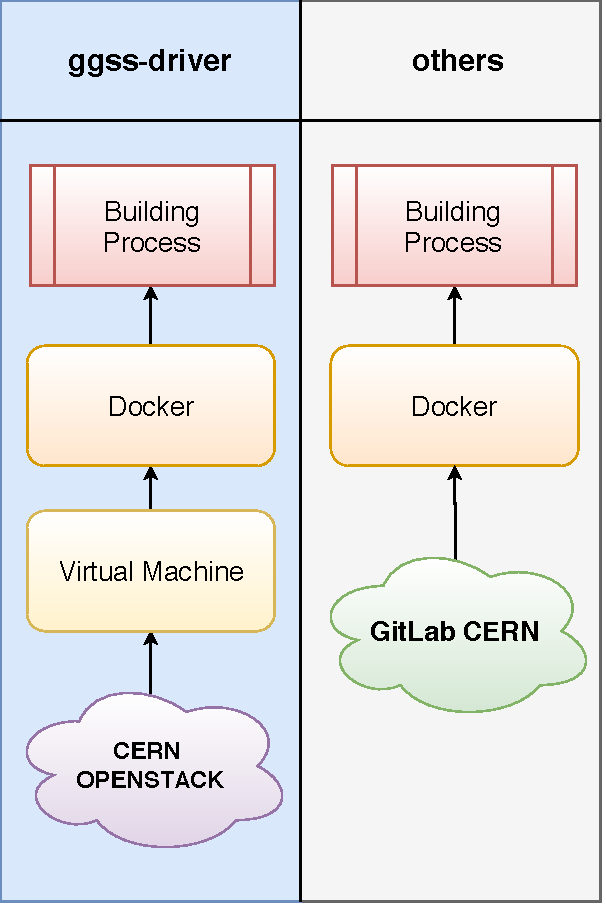
\includegraphics[width=\linewidth]{resources/buildComp}
	\end{figure}
\end{minipage}
\end{frame}


\begin{frame}
\centering{\huge{Thank You! Questions?}}
\end{frame}

\end{document}